\bchapter{Object Detection}
Al fine di comprendere a pieno e dimostrare l’utilizzo di un framework per l’implementazione di modelli di machine learning su dispositivi mobili, abbiamo
realizzato un’applicazione che ne fa uso: \textbf{ObjectDetection}.

Abbiamo scelto di utilizzare \textbf{TensorFlow} per la sua efficienza e per la maggiore disponibilità di esempi e di modelli pre-allenati di cui dispone.

L’applicazione è in grado, tramite la fotocamera frontale, di individuare e classificare gli oggetti che vede. Oltre alla classificazione, ObjectDetection
fornisce le Bounding Boxes (rettangoli) che delimitano gli oggetti e i punteggi di confidenza in merito alla sicurezza del modello sulle classificazioni fatte.
\begin{figure}
    \centering
    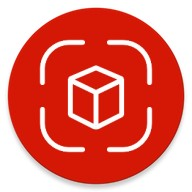
\includegraphics[width=0.3\textwidth]{Immagini/App/icona_app.jpg}
    \caption{Logo dell’app}
\end{figure}

\newpage
\section{Struttura dell'applicazione}
ObjectDetection è formata da 3 componenti principali: il primo è costituito dalle activity che si occupano di \textbf{Login} (accesso, registrazione e recupero
password), il secondo consiste in tutte le activity e le classi utilizzate per gestire la \textbf{home} dell’app e il terzo componente riguarda la gestione della
\textbf{fotocamera} e l’effettiva implementazione del modello.
L’applicazione lega e sfrutta a pieno queste 3 componenti per garantire un utilizzo scorrevole e una larga gamma di funzionalità che arricchiscono
l’esperienza dell’utente.

\subsection{Home}
La home di ObjectDetection consiste in due schermate principali: l’effettiva home e una schermata informativa (\textbf{Info}).
Una volta nella home, l’utente ha due possibilità: avviare la fotocamera e iniziare a identificare e classificare oggetti premendo sul pulsante
“\textit{Get started!}” oppure cliccare su Home aprendo un menu a tendina (\textbf{Spinner}) che fornisce le seguenti opzioni (visibili in figura \ref{fig:home}):
\begin{itemize}
    \item Info: avvia l’interfaccia informativa che fornisce dettagli sul funzionamento del modello;
    \item Change theme: cambia il tema grafico dell’applicazione; 
    \item Logout: esegui il logout dell'utente e ritorna alla schermata di Autenticazione.
\end{itemize}
\begin{figure}[H]
  \centering
  \begin{subfigure}[b]{0.3\textwidth}
    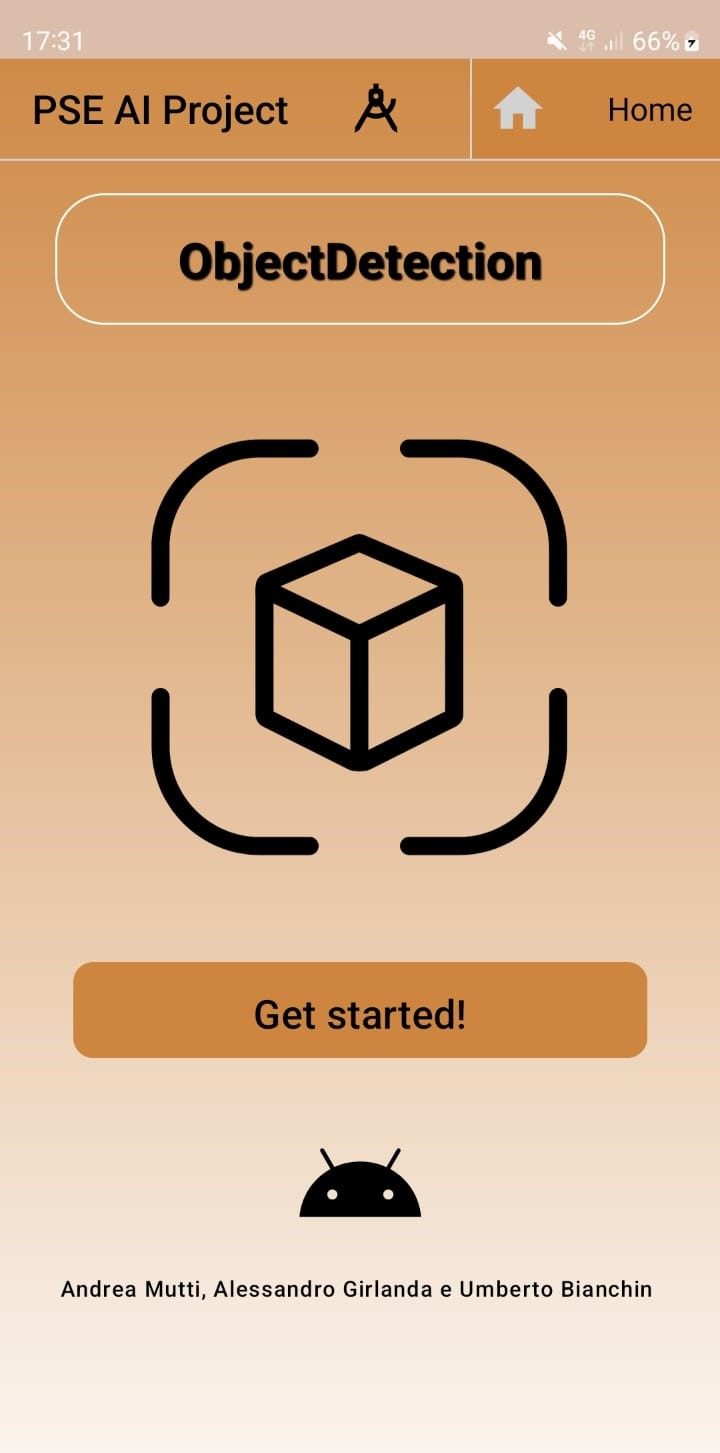
\includegraphics[width=\textwidth, height=0.4\textheight]{Immagini/App/home_chiaro.jpeg}
  \end{subfigure}
  \begin{subfigure}[b]{0.3\textwidth}
    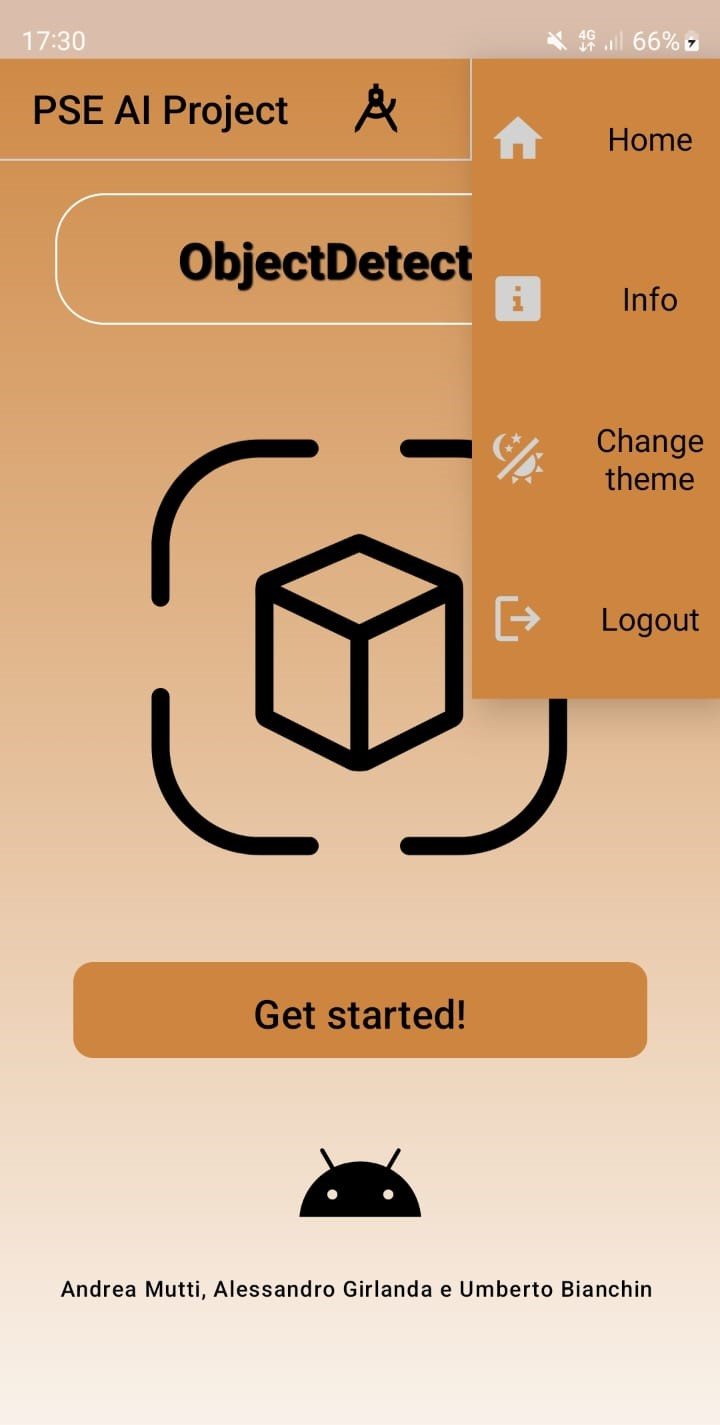
\includegraphics[width=\textwidth, height=0.4\textheight]{Immagini/App/home_spinner_chiaro.jpeg}
  \end{subfigure}
  \caption{Schermata home e apertura dello spinner.}
  \label{fig:home}
\end{figure}

\subsection{Info}
ObjectDetection fornisce una schermata informativa (Info) allo scopo di dettagliare all’utente il funzionamento dell’applicazione e del modello TensorFlow
Lite usato nell'app.
Anche in questo caso, è possibile cliccare lo spinner in alto a destra e accedere a tutte le funzionalità prima citate. Naturalmente, cliccare l’opzione
Info non comporterà alcuna azione e cliccando l’opzione Home (oppure cliccando il pulsante del proprio telefono per tornare indietro) si ritornerà alla schermata di home.

Le informazioni contenute in questa schermata (figura \ref{fig:info}) sono più di quanto essa riesca a contenere, per questo la schermata ne visualizza solo una parte e l’utente
ha la possibilità di scrollare in basso per visualizzare tutto il contenuto di questa interfaccia.

\begin{figure}[H]
  \centering
  \begin{subfigure}[b]{0.3\textwidth}
    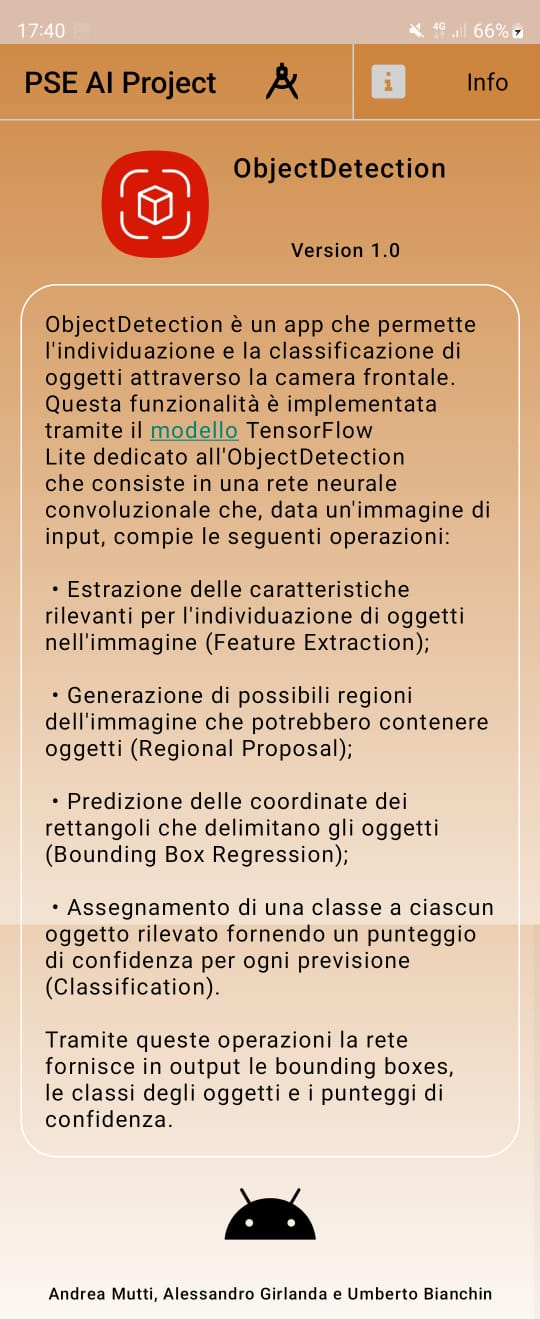
\includegraphics[width=\textwidth, height=0.45\textheight]{Immagini/App/info_chiaro.jpeg}
  \end{subfigure}
  \begin{subfigure}[b]{0.3\textwidth}
    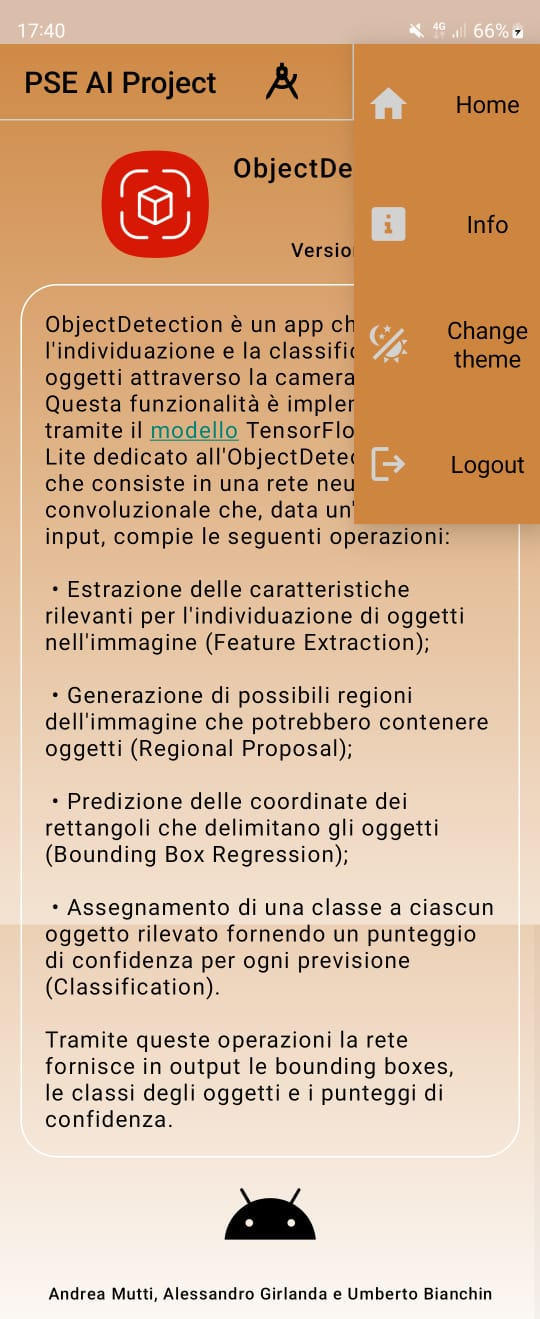
\includegraphics[width=\textwidth, height=0.45\textheight]{Immagini/App/info_spinner_chiaro.jpeg}
  \end{subfigure}
  \caption{Schermata info e apertura dello spinner.}
  \label{fig:info}
\end{figure}

\subsection{Cambio tema}
ObjectDetection fornisce, inoltre, la possibilità di cambiare il tema cromatico dell’applicazione. Fino ad ora, le schermate presentate erano tutte nel
tema \textbf{LIGHT}, realizzato in modo da essere chiaro e leggero alla vista. L’app dispone anche del tema \textbf{DARK} che presenta colori più marcati e contrastanti tra
loro (figure \ref{fig:dark1} e \ref{fig:dark2}).
Il cambio del tema si applica anche a tutti i vari widget presenti nella UI per garantire un aspetto più coerente con il tema scelto.

\begin{figure}[ht]
  \centering
  \begin{subfigure}[b]{0.3\textwidth}
    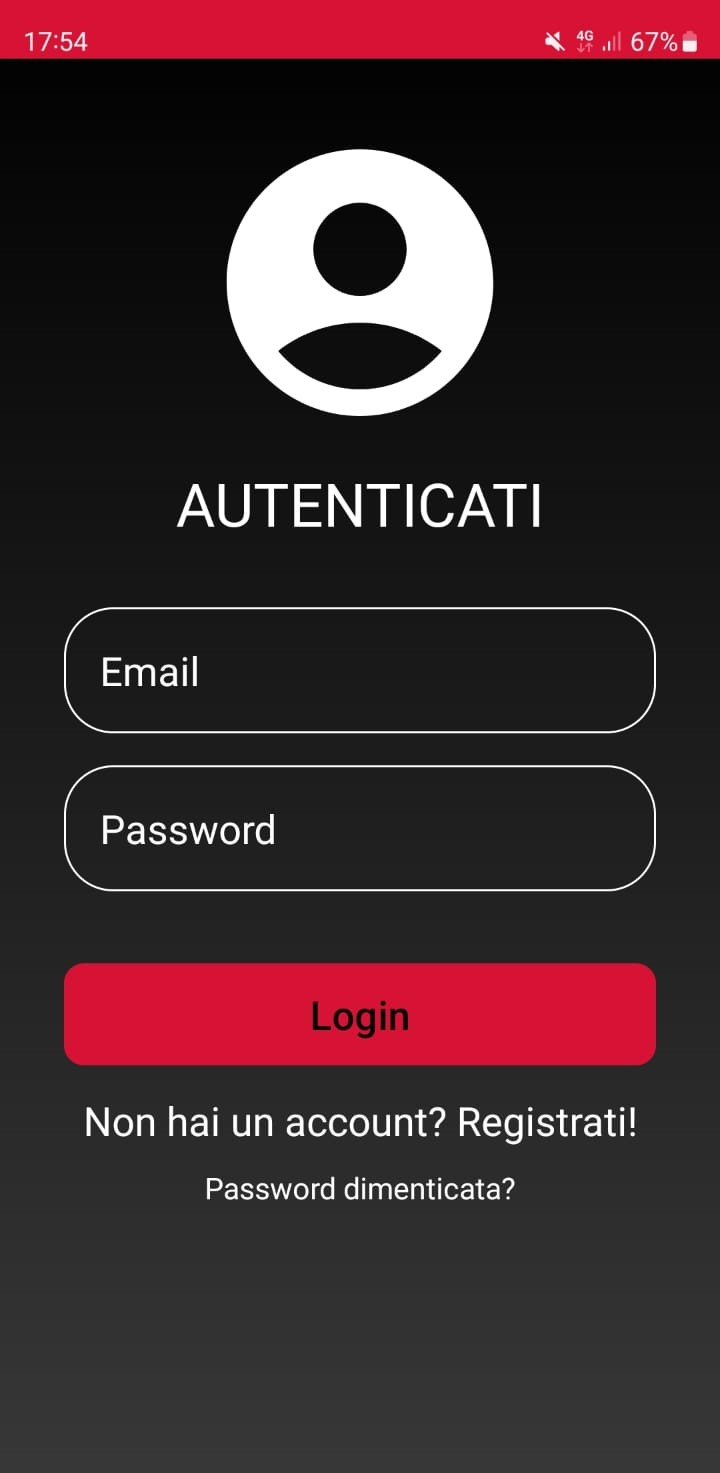
\includegraphics[width=\textwidth, height=0.4\textheight]{Immagini/App/login_scuro.jpeg}
  \end{subfigure}
  \begin{subfigure}[b]{0.3\textwidth}
    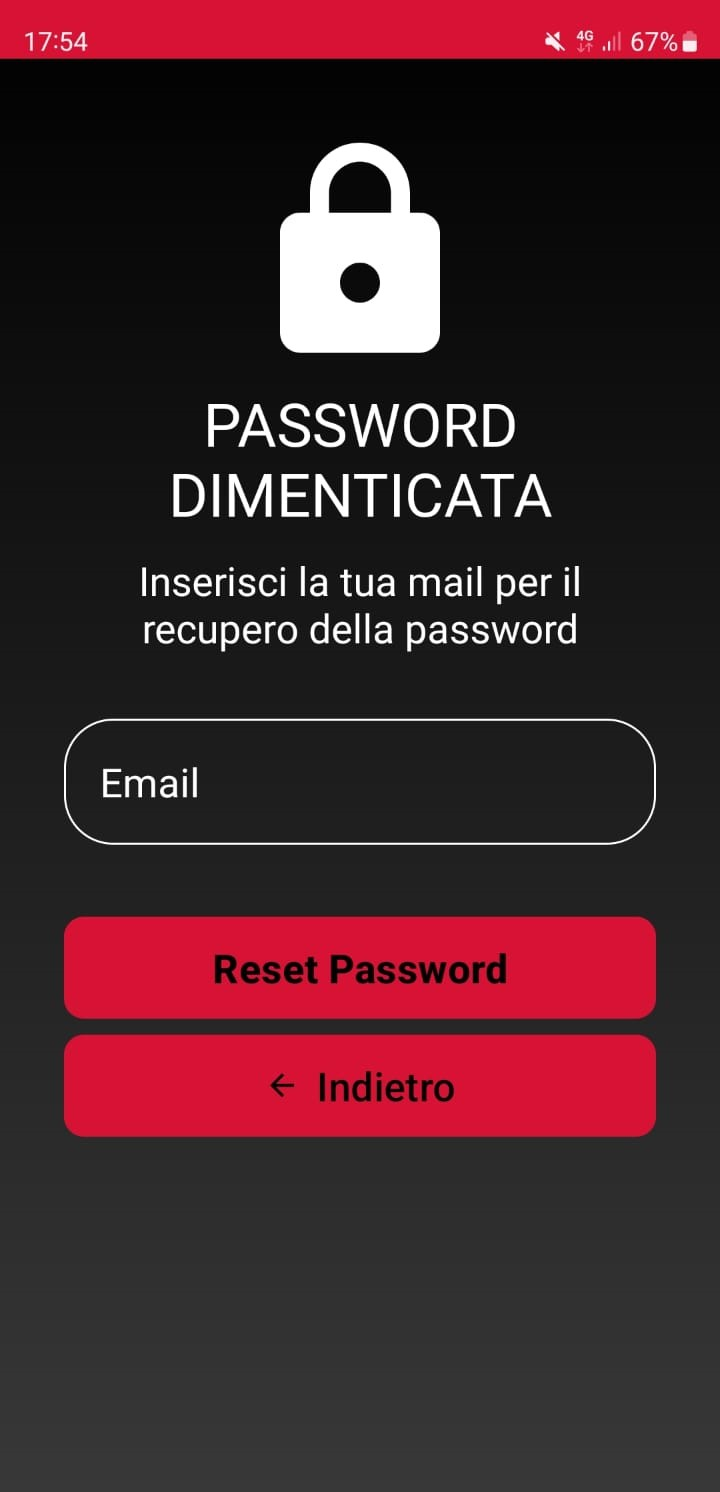
\includegraphics[width=\textwidth, height=0.4\textheight]{Immagini/App/pw_dimenticata_scuro.jpeg}
  \end{subfigure}
  \caption{Schermate di login con tema DARK.}
  \label{fig:dark1}
\end{figure}

\begin{figure}[H]
  \centering
  \begin{subfigure}[b]{0.3\textwidth}
    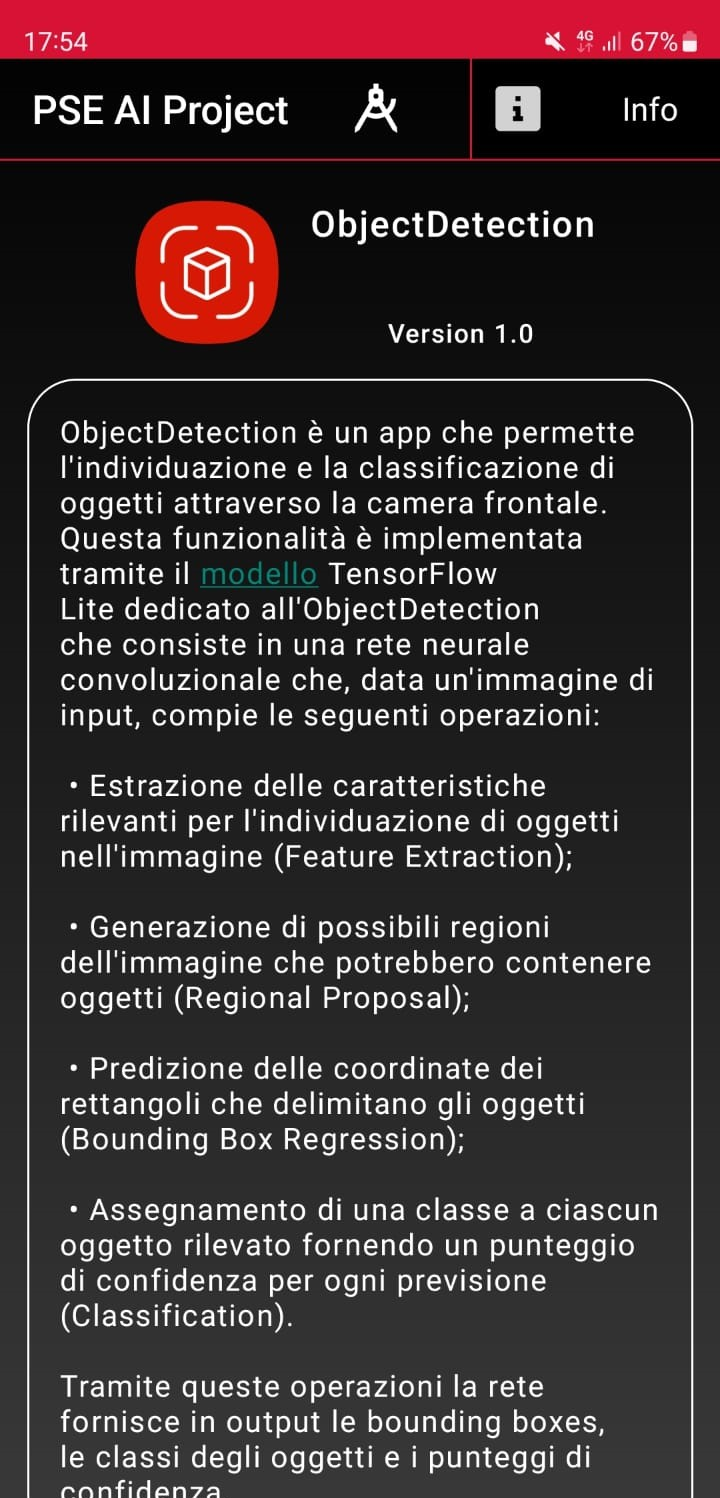
\includegraphics[width=\textwidth, height=0.4\textheight]{Immagini/App/info_scuro.jpeg}
  \end{subfigure}
  \begin{subfigure}[b]{0.3\textwidth}
    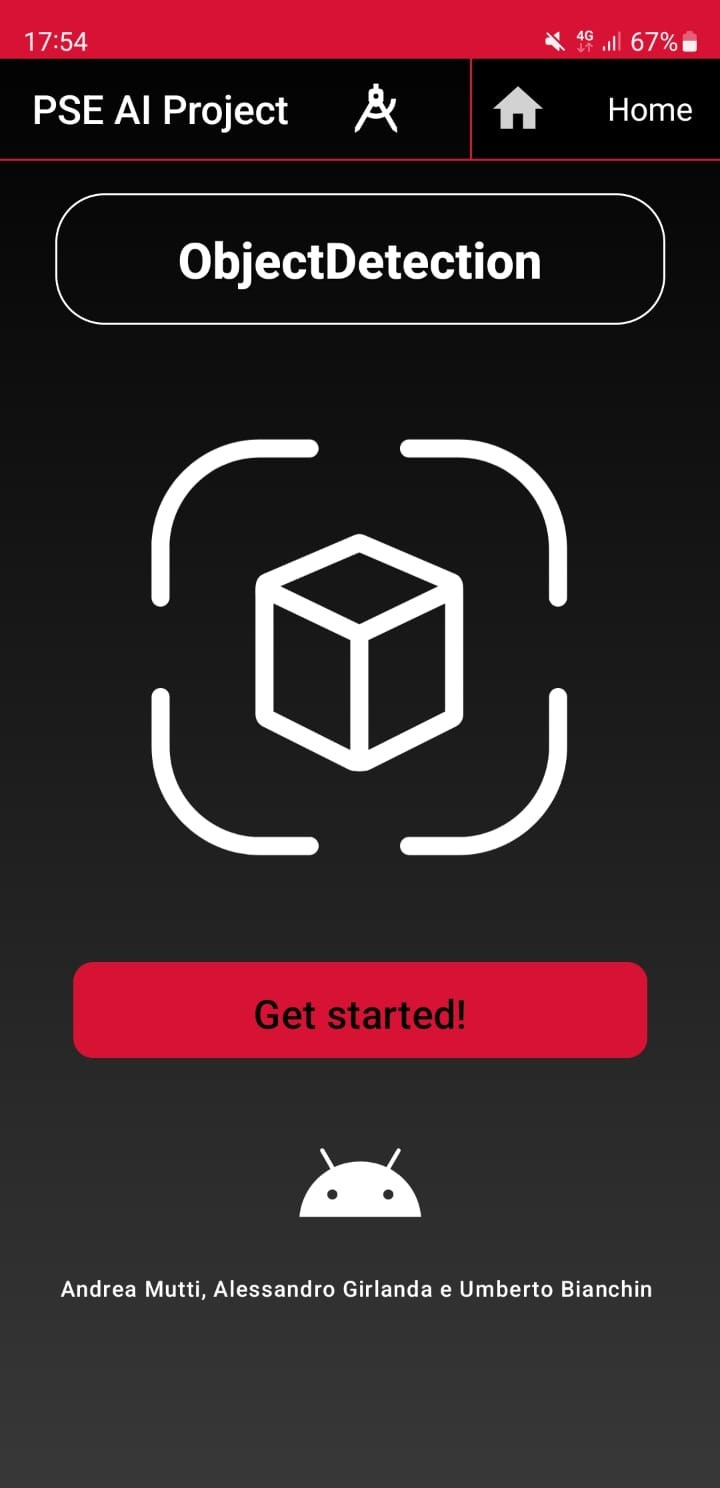
\includegraphics[width=\textwidth, height=0.4\textheight]{Immagini/App/home_scuro.jpeg}
  \end{subfigure}
  \caption{Schermate Info e Home con tema DARK.}
  \label{fig:dark2}
\end{figure}

\section{Orientamento}
In tutte le schermate dell’app, ObjectDetection supporta anche l’orientamento orizzontale completando piacevolmente l’esperienza dell’utente.
Nel cambio di configurazione, il design complessivo e le funzionalità dell’app rimangono immutate ma la disposizione e la struttura delle schermate varia
per adattarsi al nuovo orientamento del dispositivo (figure \ref{fig:orizzontale1} e \ref{fig:orizzontale2}).

\begin{figure}[H]
  \centering
  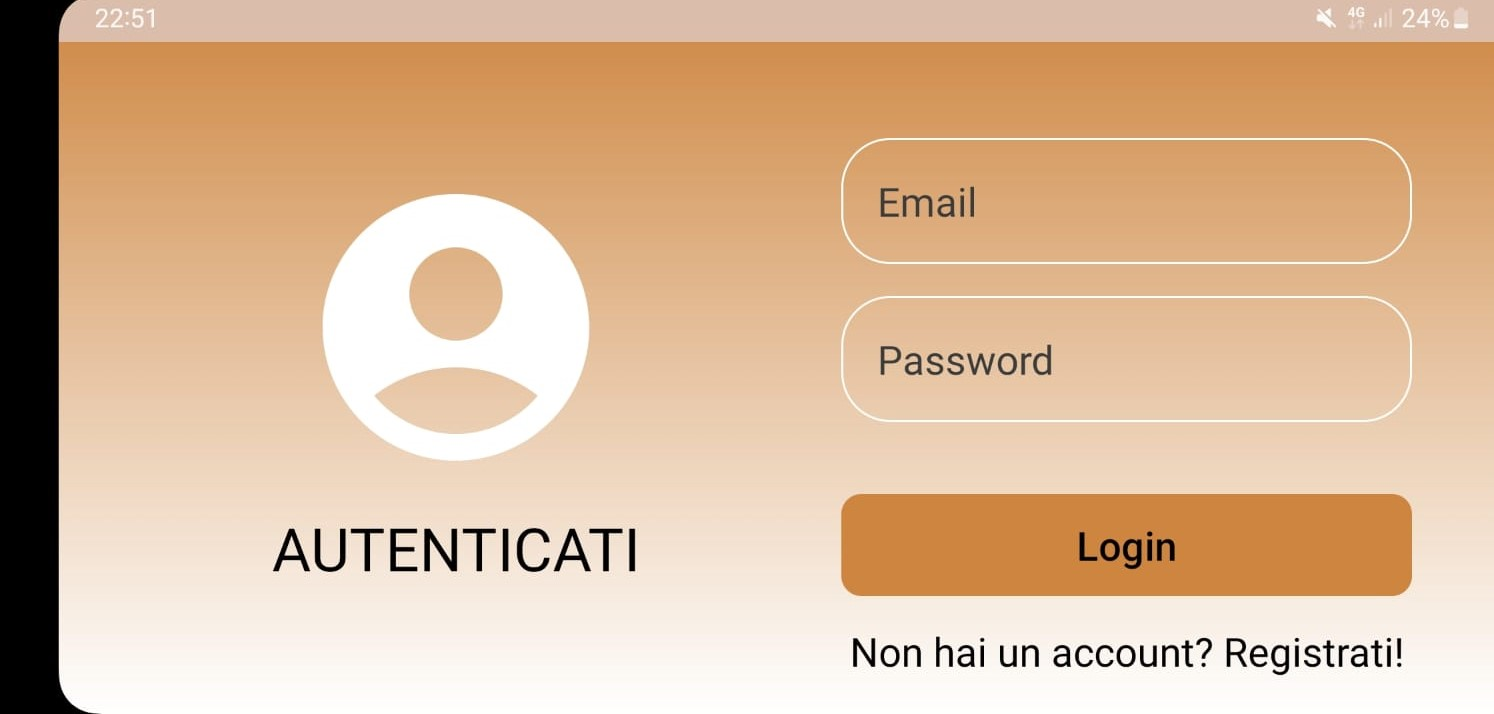
\includegraphics[width=0.5\textwidth]{Immagini/App/login_orizzontale.jpeg}
  \caption{Schermata di autenticazione con orientamento orizzontale}
  \label{fig:orizzontale1}
\end{figure}

\begin{figure}[ht]
  \centering
  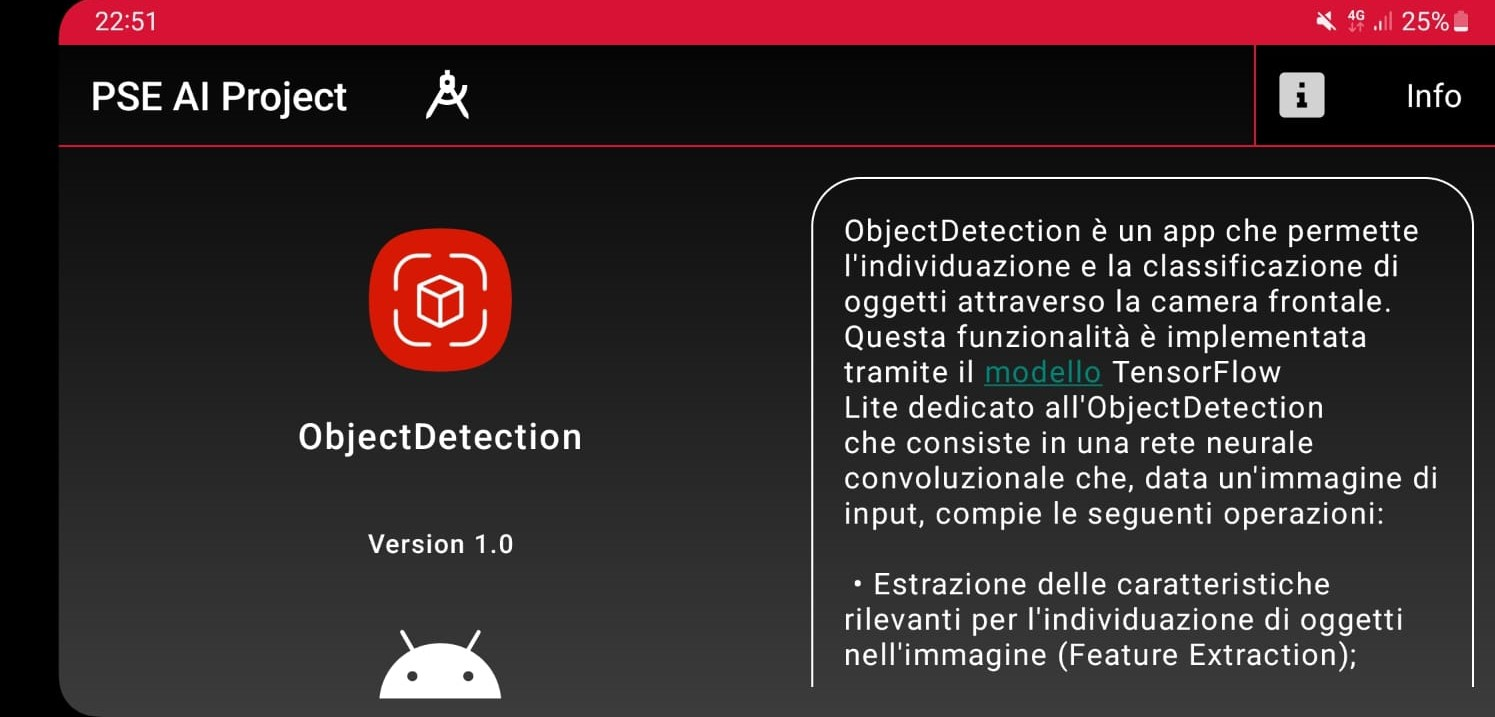
\includegraphics[width=0.5\textwidth]{Immagini/App/info_orizzontale.jpeg}
  \caption{Schermata info con orientamento orizzontale}
  \label{fig:orizzontale2}
\end{figure}

\section{Get Started!}
A seguito di questa breve descrizione strutturale, è utile mostrare alcuni esempi di utilizzo di ObjectDetection in modo da comprendere a pieno come
funziona e quali servizi offre.
Dopo aver aperto l’app ed aver effettuato il login, cliccando il pulsante “Get started!” ObjectDetection accederà alla telecamera del dispositivo (previa autorizzazione da parte dell'utente) per iniziare 
identificare oggetti.
La fotocamera usata è quella frontale e l’applicazione riconosce e classifica tutta una serie di oggetti (per i quali il modello è stato addestrato) che gli si presentano davanti.
Durante l’utilizzo dell’applicazione, è possibile aprire un menu a tendina dal basso con le seguenti opzioni:
\begin{itemize}
    \item Valore di soglia: il minimo punteggio di confidenza di cui deve disporre un oggetto classificato per mostrare la sua identificazione su schermo;
    \item Max rettangoli: il numero massimo di oggetti (e quindi di bounding boxes) che vogliamo classificare per volta. È utile per evitare che
    l’applicazione riconosca eccessivi oggetti causando un’esperienza visiva meno gradevole;
    \item Delegato: il tipo di delegato usato nell’utilizzo del modello. Si può scegliere tra CPU, GPU e NNAPI.
\end{itemize}

\begin{figure}[H]
  \centering
  \begin{subfigure}[b]{0.3\textwidth}
    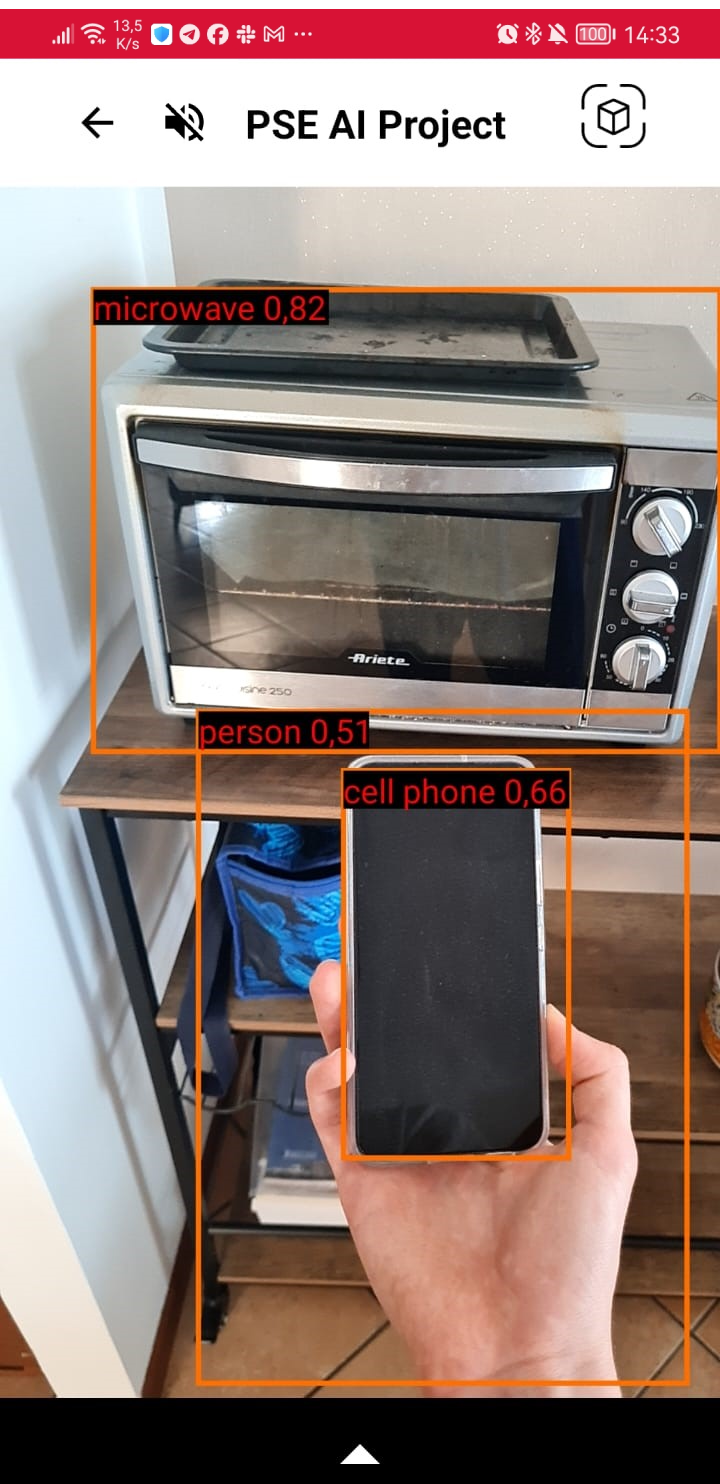
\includegraphics[width=\textwidth, height=0.45\textheight]{Immagini/App/funzionamento_3rettangoli.png}
  \end{subfigure}
  \begin{subfigure}[b]{0.3\textwidth}
    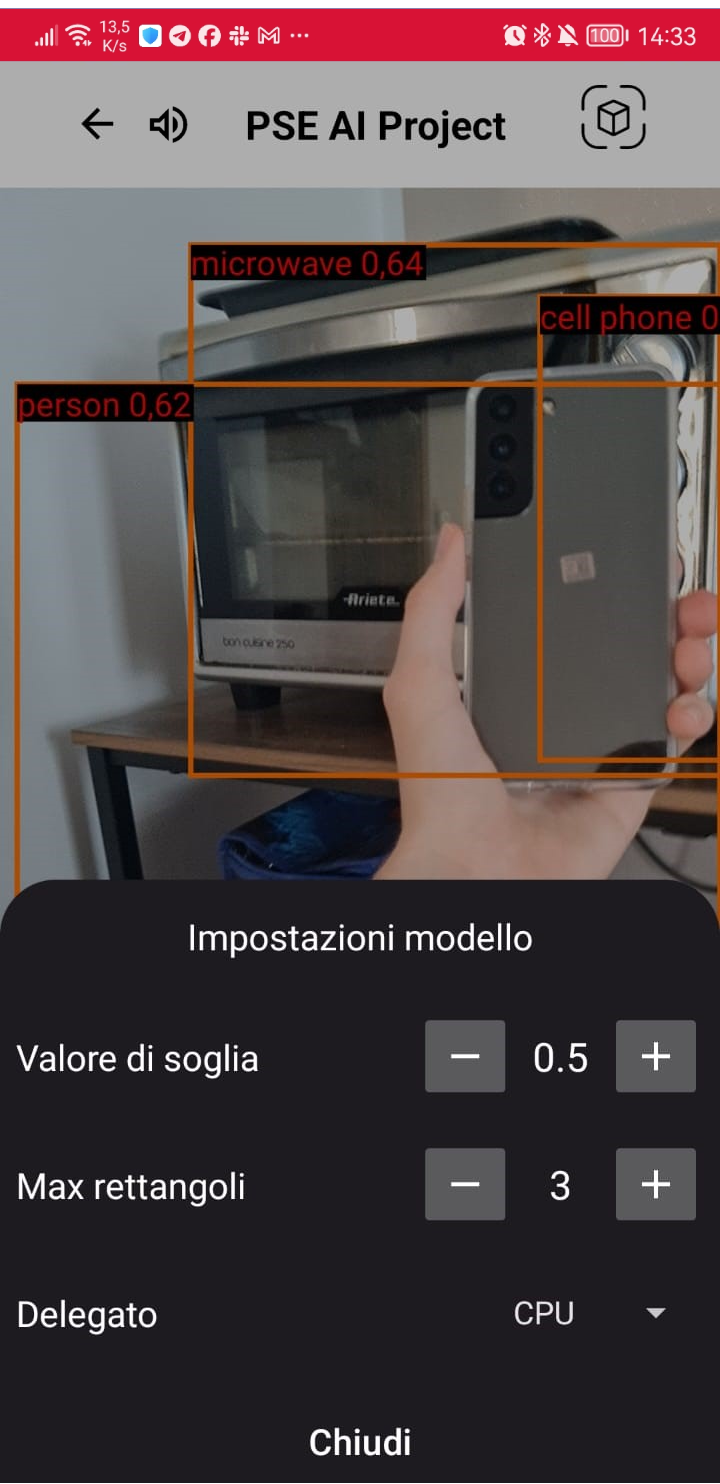
\includegraphics[width=\textwidth, height=0.45\textheight]{Immagini/App/funzionamento_impostazioni.png}
  \end{subfigure}
  \caption{Esempio di utilizzo del modello e delle sue impostazioni.}
  \label{fig:funzionamento1}
\end{figure}

Nell’esempio visibile in figura \ref{fig:funzionamento1}, l’applicazione riconosce correttamente il microonde, il telefono e la mano (classificata come persona) usando il delegato CPU.
Il numero di rettangoli massimi è 3 e il valore di soglia minimo è 0.5, infatti ciascun oggetto ha un punteggio di confidenza strettamente maggiore alla
soglia impostata.
In figura \ref{fig:funzionamento2} è possibile vedere un esempio con valore di soglia uguale ma numero massimo di rettangoli pari a 4.

\begin{figure}[H]
    \centering
    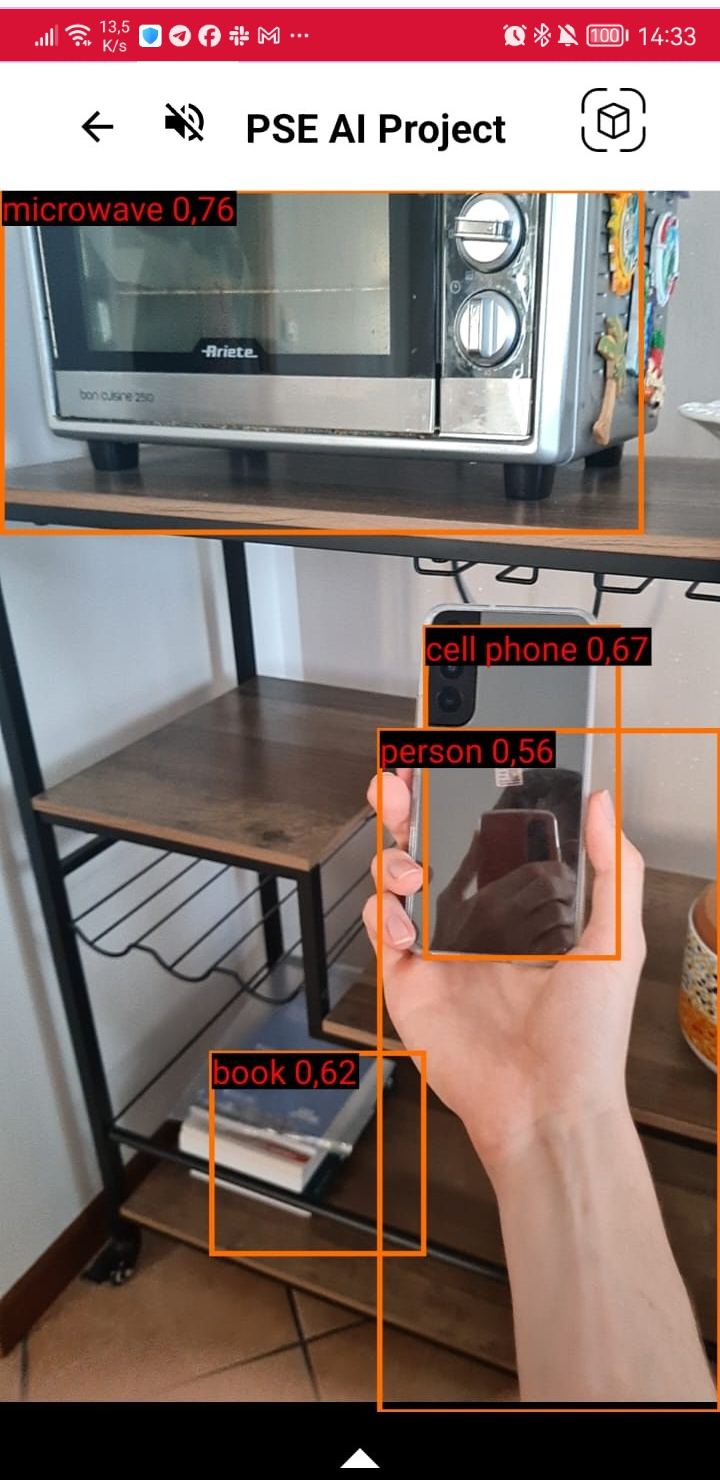
\includegraphics[width=0.3\textwidth]{Immagini/App/funzionamento_4rettangoli.png}
    \caption{Esempio di utilizzo del modello con 4 rettangoli.}
    \label{fig:funzionamento2}
\end{figure}

Come ci si aspettava, l’app riconosce correttamente quattro oggetti.
È bene notare che, in quest’ultimo esempio, il microonde non è inquadrato totalmente, il telefono è capovolto e si vede anche l’avambraccio della persona.
Tutti questi cambiamenti incidono sul punteggio di confidenza attribuito dal modello: il microonde ha un valore minore, la persona maggiore,
mentre il telefono rimane più o meno allo stesso valore.

\section{Autenticazione}
L'autenticazione della nostra applicazione è stata gestita tramite Firebase Authentication\footnote{https://firebase.google.com/docs/auth?hl=it}, che
offre una soluzione robusta e sicura per la gestione degli utenti. Grazie a Firebase Authentication, gli utenti possono registrarsi, effettuare il login
e recuperare la password in modo semplice e intuitivo. Il processo di integrazione di Firebase Authentication nella nostra applicazione è stato facilitato
dalla disponibilità di SDK e API ben documentati, che hanno permesso di implementare le funzionalità di autenticazione in modo rapido ed efficiente.


\section{Conversione modello TensorFlow a TensorFlow Lite}
Sebbene per questa applicazione sia stato utilizzato un modello TensorFlow già in versione Lite, vogliamo comunque spiegare come TensorFlow offre una
soluzione leggera e veloce per l'esecuzione di modelli di machine learning su dispositivi con risorse limitate. Una volta che si dispone di un modello
addestrato (solitamente in formato ".h5"), è necessario installare la libreria di TensorFlow nel proprio ambiente Python. Dopo di che, con un semplice 
script (codice \ref{code:1}) è possibile convertire il modello in formato ".tflite":

\begin{code}
\begin{minted}[linenos]{python}
import tensorflow as tf
    
# Carico il modello TensorFlow (Keras)
model = tf.keras.models.load_model('modello.h5')

# Creo un'istanza di TFLiteConverter
converter = tf.lite.TFLiteConverter.from_keras_model(model)

# Converto il modello
tflite_model = converter.convert()

# Salvo il modello convertito
with open('modello.tflite', 'wb') as f:
    f.write(tflite_model)
\end{minted}
\caption{Script per conversione modello TensorFlow}
\label{code:1}
\end{code}
\bigskip

Una volta effettuata la conversione, è possibile ottimizzare il modello attraverso la quantizzazione (codice \ref{code:2}) o il pruning:

\begin{code}
\begin{minted}[linenos]{python}
# Abilitare la quantizzazione
converter.optimizations = [tf.lite.Optimize.DEFAULT]

# Convertire il modello con quantizzazione
tflite_quantized_model = converter.convert()

# Salvare il modello quantizzato
with open('modello_quantizzato.tflite', 'wb') as f:
    f.write(tflite_quantized_model)
\end{minted}
\caption{Script per quantizzazione del modello}
\label{code:2}
\end{code}

\section{Modello}
Il modello utilizzato nell'applicazione è una componente fondamentale per il rilevamento degli oggetti e si tratta di un modello di tipo Object Detection.
È importante sottolineare che questo modello è pre-allenato, il che significa che è stato precedentemente addestrato su un ampio set di dati per riconoscere
una vasta gamma di oggetti. Ciò consente all'applicazione di identificare oggetti in tempo reale attraverso la fotocamera del dispositivo.
Sebbene il modello fosse già disponibile come esempio in TFLite, abbiamo riscritto da zero il codice per adattarlo alle nostre esigenze specifiche e
garantire un'integrazione senza problemi con l'interfaccia utente dell'applicazione. Inoltre il codice fornito con l’esempio risultava ad oggi obsoleto.

L'interfaccia fornita dal modello è progettata per essere intuitiva e semplice da utilizzare. L'unico tipo di input supportato è un'immagine Bitmap con
dimensioni di 300 x 300 pixel e tre canali per pixel (RGB). È importante notare che i valori dei pixel nell'immagine sono di tipo uint8, ovvero valori
senza segno su 8 bit che variano da 0 a 255.
Tuttavia, le fotocamere dei dispositivi moderni possono raggiungere risoluzioni molto più elevate, come il formato 4K (3840 x 2160) o almeno in HD. Di
conseguenza, abbiamo dovuto implementare una logica per convertire l'immagine catturata dalla fotocamera in un formato compatibile con le dimensioni di
input richieste dal modello, cioè 300 x 300 pixel.

Una delle caratteristiche chiave del modello è la possibilità di selezionare il delegato da utilizzare per l'esecuzione delle inferenze. Di default, il
delegato utilizzato è il processore (CPU), ma è possibile cambiare questa impostazione tramite una finestra a tendina nell'interfaccia utente
dell'applicazione. I delegati disponibili includono CPU, GPU e NNAPI (Android Neural Networks API), che offrono prestazioni e ottimizzazioni specifiche
per il dispositivo in uso.
È importante sottolineare che l'applicazione è progettata per gestire eventuali errori o incompatibilità durante l'utilizzo dei diversi delegati per
l'esecuzione del modello. Se il delegato selezionato non è supportato sul dispositivo in uso, verrà visualizzato un messaggio di errore, ma l'applicazione
continuerà a funzionare senza interruzioni. In particolare, la scelta di un delegato non utilizzabile, comporta il ripristino dopo circa un secondo del
delegato base, ovvero CPU. Questo garantisce un'esperienza utente fluida e affidabile anche in condizioni non ideali.

Inoltre, nell'interfaccia utente della fotocamera, è presente un overlay fisso che mostra i risultati del rilevamento degli oggetti. Questi risultati sono
rappresentati da rettangoli posizionati sull'immagine in base alla posizione degli oggetti rilevati. Ogni rettangolo è accompagnato da informazioni sulla
categoria dell'oggetto e il punteggio di confidenza associato.

Per garantire una visualizzazione accurata dei risultati, è necessario applicare un fattore di scala per adattare le coordinate dei rettangoli dalla
dimensione della bitmap utilizzata dal modello alla dimensione effettiva dell'immagine catturata dalla fotocamera. Questo processo assicura che i rettangoli
siano correttamente sovrapposti all'oggetto rilevato nell'immagine visualizzata e che non siano presenti rettangoli che fuoriescono dai bordi imposti dallo
schermo, in modo da renderli sempre totalmente leggibili.

Inoltre, l'applicazione offre la possibilità di personalizzare la soglia di confidenza per il rilevamento degli oggetti e il numero massimo di risultati da
visualizzare contemporaneamente. Anche queste impostazioni possono essere regolate dall'utente tramite la finestra a tendina nell'interfaccia utente e
vengono salvate per essere applicate automaticamente ad ogni avvio dell'applicazione.
Ogni modifica viene salvata in una SharedPreference che permette il salvataggio e il ripristino delle scelte ad ogni avvio dell’app.

Per garantire una forte user experience è stato adottato un controllo sui risultati presenti. In particolare, se i risultati ottenuti non cambiano, ovvero
rimangono intatti come numero e come classi ottenute, allora la visualizzazione viene modificata solo ogni secondo. Nel momento in cui è presente una classe
in più o in meno o ci sono differenze, viene aggiornata la visione. Questo permette di non vedere troppe informazioni in continua modifica a schermo. Il
tutto è realizzato tramite l’utilizzo di un timer non bloccante e un semplice controllo in retroazione.

Infine, per aumentare l’accessibilità dell’applicazione, è stata aggiunta un’icona di volume on/off nella parte alta della toolbar durante l’utilizzo
della fotocamera. Premendo il pulsante è possibile attivare o disattivare il TextToSpeech che dà informazioni sugli oggetti trovati e il relativo
punteggio. Si tratta sia di un miglioramento a livello UX, sia un miglioramento tecnico dell’applicazione, per poter aumentare la sua utilità.

In figura \ref{fig:modello} si può vedere l’immagine che descrive I/O del modello.

\begin{figure}[ht]
    \centering
    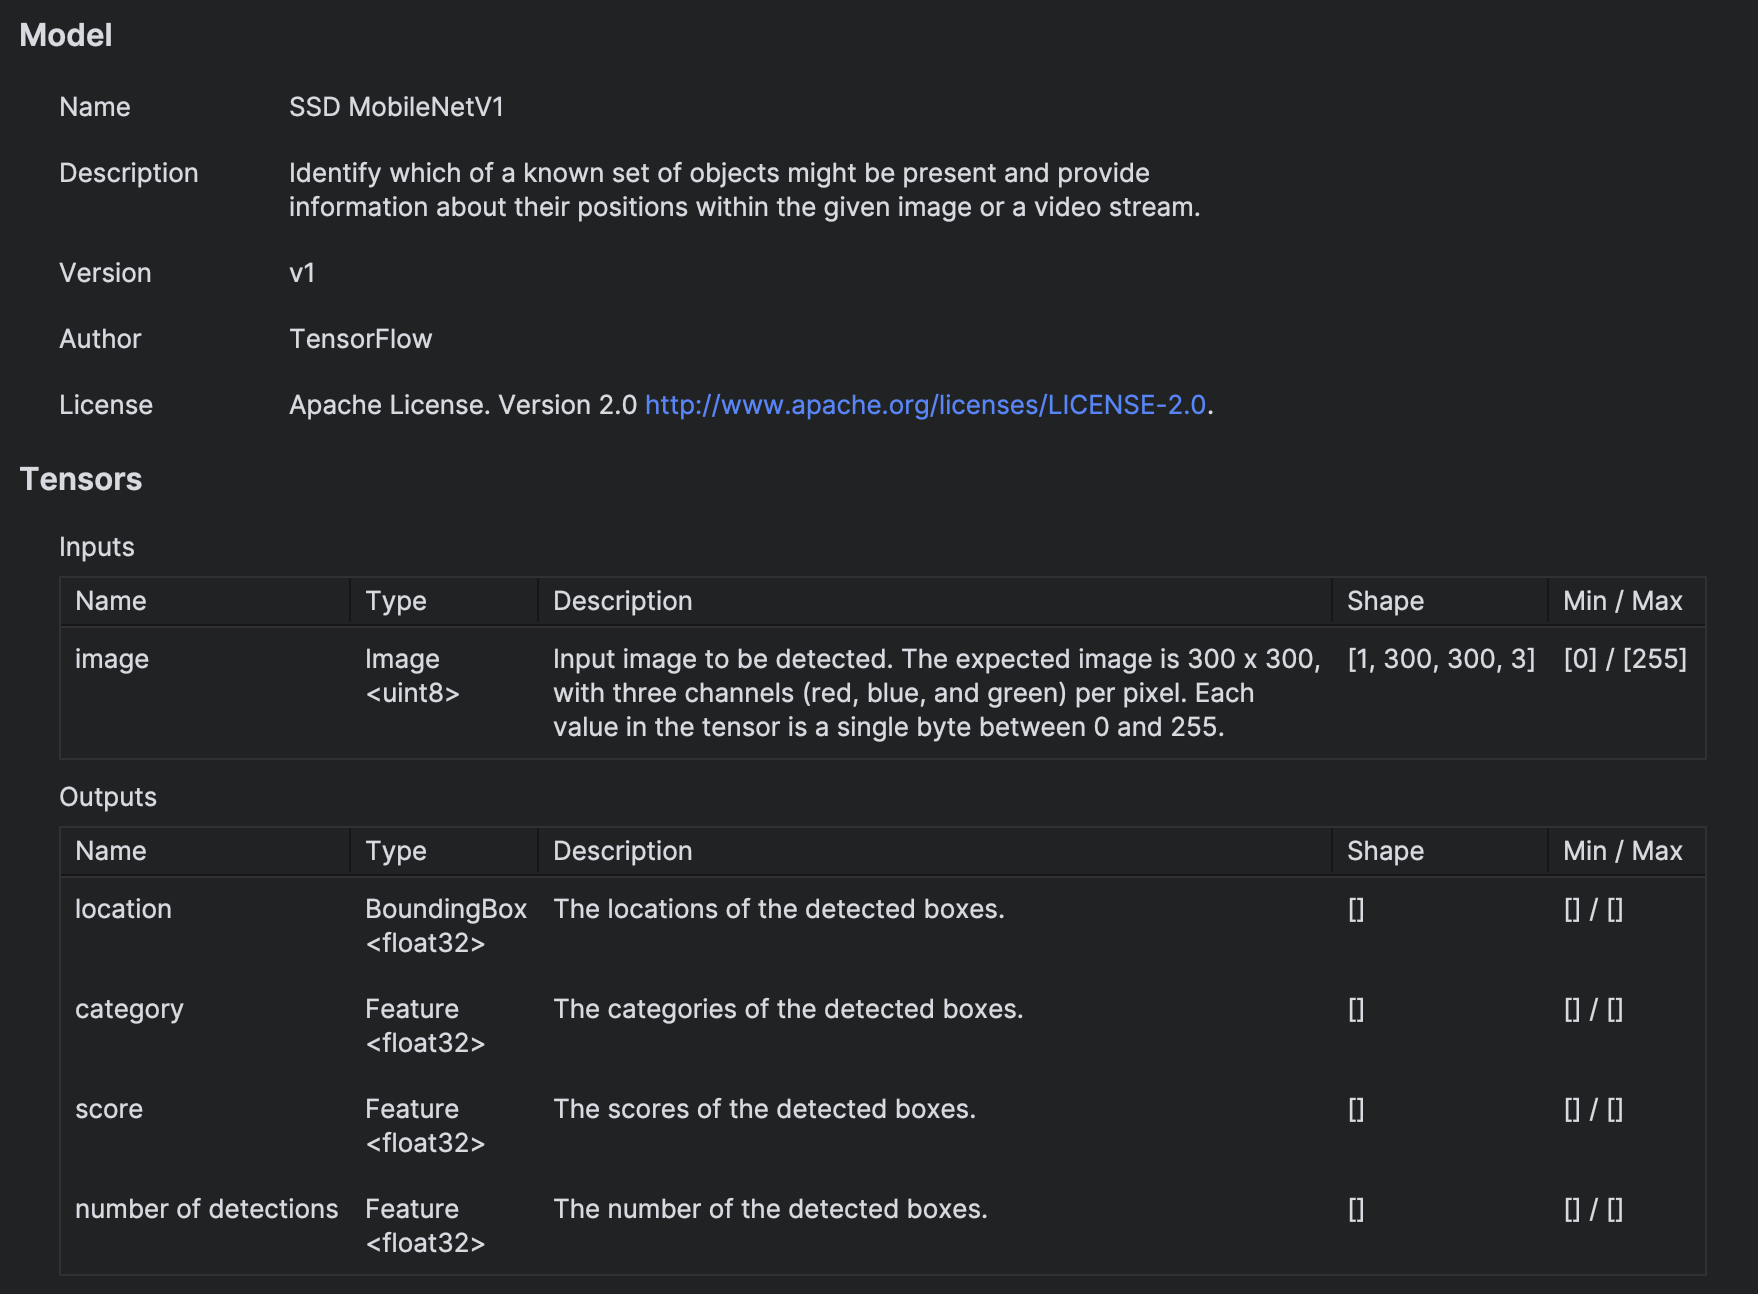
\includegraphics[width=0.8\textwidth]{Immagini/App/modello.png}
    \caption{I/O del modello}
    \label{fig:modello}
\end{figure}
